\section{Motivation}
Modern day technology has developed under incredible speed in recent decade and the computing power growth rate is truly phenomenal and lasting impact can be felt and benefit us in many ways. It is important to realise the worldwide effect on environment by the increase in consumption of power by these technology advancements.

According to~\cite{pickavet2008worldwide}, the power consumption growth rates of PCs are about 7.5\% per year. Data Centres and network play much larger role as they both have power consumption rate of 12\% each. This considerable growth is due to increasing data to be accessed, stored and processed. This constant expansion of energy consumption leads to increase in carbon emissions. \(CO_2\) emissions from ICT (Information and communications technology) are increasing at a rate of 6\% per year, at such rate by 2020 it will account to 12\% of worldwide emissions ~\cite{rong2016optimizing}.

\begin{figure}[ht]
	\centering
	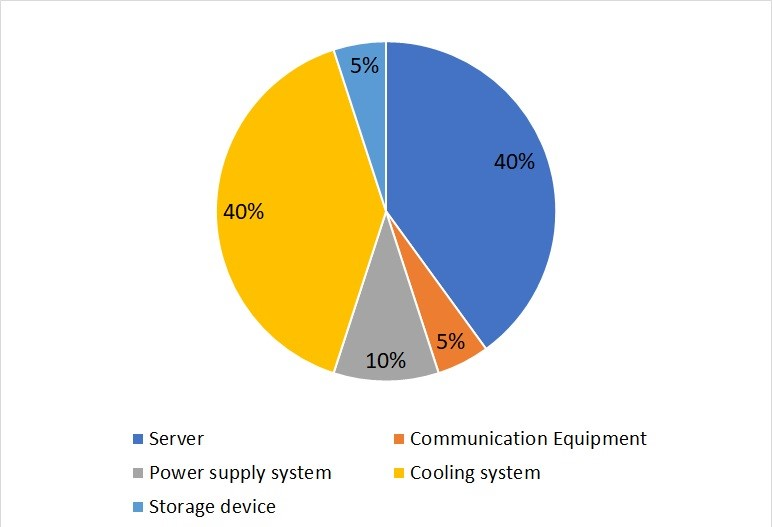
\includegraphics[width=200pt]{energypiechart}
	\caption{\label{fig:energypie} Energy consumption distribution of data centers.}
\end{figure}

The major roles of power consumption by a data ware house is played by the servers and the cooling system which is used to cool down the server physical parts. From the figure~\ref{fig:energypie}, you can see they both account to 80\% of the total consumption with both accounting for 40\% each~\cite{rong2016optimizing}. Hence by finding a relation between different events and energy consumption, we could minimize the power consumption by the systems. Minimising energy consumed will also decrease the heat generated by the system which will in turn lower down the usage of cooling system. Leading us to minimise cost and save environment.

Thus, if we could discover the functional relational between the demand of the power and the performance events (PMCs), that could enable us the ability to adjust, and predict the energy consumption for certain computations.

\section{Aims}

The projects aim is to create a piece of software that is extensible, easy to use and performant. A tool that can perform analyses like regression and clustering and give us an overview of the data by show casing the relationship of various parameters with the output. In this case, our parameters are the performance events and output is the energy consumption. Following are the objectives that we want to achieve.

\subsection{Existence of functional relation}

Datasets are mostly pair of multiple inputs and a single output. And the possibility of the existence is what we are interested in. Is it possible to define the data in a form of function? Question like this is one of the aims. Defining the data in a form of function is explaining the dataset in a form of a formula which can combine various parts of the input parameters and give the output. It is quite impossible to tell that whether a function definetly exists as the data we have is always a subset and there are number of records which are either not in the dataset or we donot know. But, regardless we can definitely explain the non-existence of a formula by finding a pair of input parameters and outputs that violate the definition of a function.

The pair which violates the definition of a function must be looked at as there is high probability of that data set record being corrupt or if not it can actually help and tell the non existence. If this outlier is in fact corrupt, this process can be used for data cleanups as well.

\subsection{Analysis of functional relation}

Once, we are no more able to prove functional non existence in the dataset. We can try to analyse the dataset and try to examine the various relations of the parameters with the output. Analysis of the parameters with output is done to know how much change in one parameter contributes to the change in the output. This analysis helps us to understand the correlation between two quantities. Does high page faults correlates to high energy consumption? Questions like this is what the analysis of parameters with their corresponding output answers. This can also be thought of an explaination of the output parameters.

In other words, understanding the correlation is the other aim. Once we are able to know that there is high correlation. We can then dig deep into the data and try to find out the reason for the same.

\section{Approach}

For each of the aims, two approaches have been employed. Both the approaches tries to achieve the same conclusions with different methodology.

The experimental data sets provided has the following format:

\(E_1,\ x_{11},\ x_{12},\ x_{13} \ldots x_{1k}\)\\
\(E_1,\ x_{21},\ x_{22},\ x_{23} \ldots x_{2k}\)\\
\ldots \\
\(E_n,\ x_{n1},\ x_{n2},\ x_{n3} \ldots x_{nk}\)

where \(k\) is the total number of parameters (performance events), \(n\) is the number of records in the dataset.
\(E_i\) is the experimentally obtained dynamic energy consumption and \(x_{ij}\) are the experimentally obtained performance events (PMCs).

\subsection{Existence of functional relation}

Our main goal here is to find nonexistence of functional relationship. In other words, it means proving that the dataset cannot be explained in terms of a function/formula.

Our first approach here is to find two performance events tuples \((x_{i1},\ x_{i2},\ x_{i3} \ldots x_{ik})\) and \((x_{j1},\ x_{j2},\ x_{j3} \ldots x_{jk})\) are equal within some tolerance, but their corresponding \(E_i\) and \(E_j\) dynamic energy consumption is different. Existence of such a tuple in database will lead us to prove the non-existence of a functional relationship.

It is infact easier to find two equal records by ordering the dataset by their parameters and going through the entire dataset once to find equal records and comparing their dynamic energy consumption. The order of complexity is O(N log N) which is the complexity of sorting as that is the only heavy duty task involved. But it gets really complicated when tolerance comes into play. In other words, we have to find similar records than equal records. The project employs 2 methods to measure the similarity between the two data records.

First approach:

The data records are imagined as data points in \(k-space\) as we have \(k\) number of parameters. Then we divide the whole space into small \(k-dimension cubes\) whose dimensions \((t_1, t_2, \ldots t_k)\) where \(t_i\) is the tolerance of each parameter. The data points are then put in their respective cubes. And each cube is then analysed to see that whether the data points output are similar to each other as well.

Second approach:

The data points in \(k-space\) are similar if the euclidean distance between them is less than the \(t\) provided, where \(t\) is the total/max tolerance. Data points which are infact found to be close to each other, their output is compared to see if they are similar to each other.

\subsection{Analysis of functional relation}

Many different type of relations can be there between two variables. But, we are interested in more general trend of the dynamic energy consumption output with the performance events. Many researches have used linear models, to understand the relation between energy consumption and performance events.\cite{o2017survey} And this is due to the trickle down effect of the relation.\cite{bircher2007complete} Hence, we also used linear regression to analyse the relationship.

Linear regression is done with 2 variables but we have \(k\) variables relation to energy consumption making it hard to understand the nature. Hence to analyse one of the variable we have to isolate it in the space where the other \(k-1\) variables donot change. Data points are clustered using \(k-1\) variables. Each cluster is then visited and linear regression is performed. Two approaches are employed to cluster which are similar to finding similar records in finding the existence of the relation.

First approach:

Data points are clustered by putting the data points in the respective \(k-1 dimension cube\). Forming a cluster with almost similar \(k-1 variables\).

Second approach:

Euclidean distance is used to isolate similar \(k-1 variables\). A \(k-1 dimension sphere\) can be imagined for simplicity with its radius being the total/max tolerance.

In both approaches, linear regression is performed on the cluster with the variable which was not used in clustering and the output which is the dynamic energy consumption.

Above is just only one field that possible usage of the functional relationship in data. In real world there are much more application that required such technique. Such as hybrid vehicle power management, power supply of auxiliary power units etc. There are many past work in this field but only few were focus on the relationship between dynamic energy consumption and PMCs. Hence, in this report we will try to observe the relationship between energy consumption and PMCs. We will explore the monotonicity of the relationship between dynamic energy consumption and performance events (PMCs) and suggesting the non-existence of a functional relationship as well.

\section{Structure of report}
In this report, you must have already seen the motivation behind the project and brief description of the approaches that will be taken to reach the objective.

This Introductory chapter is followed by Background research, design aspects of the software, implementation of the software, testing and evaluation of the tool followed by the conclusion and the future works.

Background research explains about performance events and how do they influence energy consumption by the system. It also explains the approaches in detail mentioned above and analyses their complexity and how they can be optimised.

Following Background research, design and implementation of the software is deep dig into as we want an extensible, performant tool. Testing and evaluation of the software is explained. How the software is tested and its evaluation on its performance. The report ends with conclusions and future works that shows how the project can be extended and applied to various other domains.